\documentclass{article}
\usepackage{marvosym}

%...TikZ & PGF
\usepackage{pgfplots}
\pgfplotsset{compat=1.11}
\tikzset{>=latex}
\usetikzlibrary{calc,math}
\usepackage{tikzsymbols}
\usepgfplotslibrary{fillbetween}
\usetikzlibrary{decorations.markings} 
\usetikzlibrary{arrows.meta} %...APP2 for arrows as objects and images
\usetikzlibrary{backgrounds} %...For shading portions of graphs
\usetikzlibrary{patterns} %...Unit 5 Problems
\usetikzlibrary{shapes.geometric} %...For drawing cylinders in Unit 2
\usepackage{makecell} %...use \thead{} to enable line skip in table headers
\tikzset{
    mark position/.style args={#1(#2)}{
        postaction={
            decorate,
            decoration={
                markings,
                mark=at position #1 with \coordinate (#2);
            }
        }
    }
} %...See https://tex.stackexchange.com/questions/43960/define-node-at-relative-coordinates-of-draw-plot

\tikzset{
    declare function = {trajectoryequation10(\x,\vi,\thetai)= tan(\thetai)*\x - 10*\x^2/(2*(\vi*cos(\thetai))^2);},
    declare function = {trajectoryequation(\x,\vi,\thetai)= tan(\thetai)*\x - 9.8*\x^2/(2*(\vi*cos(\thetai))^2);},
    declare function = {patheq(\x,\yi,\vi,\thetai)= \yi + tan(\thetai)*\x - 9.8*\x^2/(2*(\vi*cos(\thetai))^2);},
    declare function = {patheqten(\x,\yi,\vi,\thetai)= \yi + tan(\thetai)*\x - 10*\x^2/(2*(\vi*cos(\thetai))^2);} %like patheq but with gravity = 10
}

%...siunitx
\usepackage{siunitx}
\DeclareSIUnit{\nothing}{\relax}
\def\mymu{\SI{}{\micro\nothing} }
\DeclareSIUnit\mmHg{mmHg}
\DeclareSIUnit{\mile}{mi}
%...NOTE: "The product symbol between the number and unit is set using the quantity-product option."

%...Other
\usepackage{amsthm}
\usepackage{amsmath}
\usepackage{amssymb}
\usepackage{cancel}
\usepackage{subcaption}
\usepackage{dashrule}
\usepackage{enumitem}
\usepackage{fontawesome}
\usepackage{multicol}
\usepackage{glossaries}
%\numberwithin{equation}{section}
\numberwithin{figure}{section}
\usepackage{float}
\usepackage{twemojis} %...twitter emojis
\usepackage{utfsym}
\usepackage{linearb} %...For \BPwheel in Unit 8
\newcommand{\R}{\mathbb{R}} %...real number symbol
\usepackage{graphicx}
\graphicspath{ {../Figures/} }
\usepackage{hyperref}
\hypersetup{colorlinks=true,
    linkcolor=blue,
    filecolor=magenta,
    urlcolor=cyan,}
\urlstyle{same}
\newcommand{\hdashline}{{\hdashrule{\textwidth}{0.5pt}{0.8mm}}}
\newcommand{\hgraydashline}{{\color{lightgray} \hdashrule{0.99\textwidth}{1pt}{0.8mm}}}

%...Miscellaneous user-defined symbols
\newcommand{\fnet}{F_{\text{net}}} %...For net force
\newcommand{\bvec}[1]{\vec{\mathbf{#1}}} %...bold vector
\newcommand{\bhat}[1]{\,\hat{\mathbf{#1}}} %...bold hat vector
\newcommand{\que}{\mathord{?}}  %...Question mark symbol in equation env
%...Define thick horizontal rule for examples:
\newcommand{\hhrule}{\hrule\hrule}
\let\oldtexttt\texttt% Store \texttt
\renewcommand{\texttt}[2][black]{\textcolor{#1}{\ttfamily #2}}% 

%...For use in the exam document class
\newif\ifprintmetasolutions


%...Decreases space above and below align and gather enironment
\makeatletter
\g@addto@macro\normalsize{%
  \setlength\abovedisplayskip{-3pt}
  \setlength\belowdisplayskip{6pt} 
}
\makeatother





\usepackage[margin=1in]{geometry}
\usepackage{OutilsGeomTikz}

%...Theorem for examples
\theoremstyle{definition}
\newtheorem{example}{Example}
\newtheorem{exercise}{Exercise}

%...Define colors for use in Unit 11: SHM and Waves
\pgfdeclarehorizontalshading{visiblelight}{50bp}{
color(0.00000000000000bp)=(red);
color(8.33333333333333bp)=(orange);
color(16.66666666666670bp)=(yellow);
color(25.00000000000000bp)=(green);
color(33.33333333333330bp)=(cyan);
color(41.66666666666670bp)=(blue);
color(50.00000000000000bp)=(violet)
}

\setlength\parindent{0pt}
\setlength{\parskip}{6pt}

\renewcommand{\thesubsubsection}{\thesubsection\alph{subsubsection}}
\begin{document}

\begin{center}
    \textbf{Unit 1: Constant Motion}
\end{center}

\section{Position, Distance, and Displacement} \label{pdfqW3}


Physical objects---like a person, an asteroid, or an electron---move through physical space. To trace and describe their motion, we use physical properties like position, speed, and acceleration. \relax{position} ($d$) is the location of an object on a fixed axis.

\begin{center}
    \begin{tabular}{cl|cl}
    \hline
    \textbf{Symbol} & \textbf{Quantity} & \textbf{SI Unit} & \textbf{Unit Symbol}  \\
    \hline\hline
        $d$ & position & meter & m\\
    \hline
    \end{tabular}
\end{center}

\begin{example} \label{xNmqo7}
    Consider the position axis below. (a) What is the position of the stick figure? (b) What is the position of the house? (c) What is tree's position? 
\end{example}

\begin{center}
    \begin{tikzpicture}
    \begin{axis}[width=15cm,
        axis lines = left,
        axis y line=none,
        xlabel = {Position (m)},
        ymin=0, ymax=12, 
        xmin=-10, xmax=10,
        xtick={-10,-8,...,12},
        clip=false,
        ]
        \node[above] at (-8,0) {\Springtree[3]};
        \node[above] at (8,0) {\huge \faHome};
        \node[above] at (0,0) {\Strichmaxerl[2.5]} ;
    \end{axis}
    \end{tikzpicture}
    \captionsetup{type=figure,margin=1in,font=scriptsize}
    \captionof{figure}{A position axis with a person at the origin and a tree and house at different positions.}
\end{center}

 We read the axis to specify the position of objects. (a) The stick figure's position is zero meters. (b) The house's position is $d = \SI{8}{meters}$. (c) The tree's position is $d = \SI{-8}{m}$.

\hrule    

\vspace{1em}

% \vspace{1em}

% \hrule

% \vspace{1em}

If the person in Example~\ref{xNmqo7} moves from the origin to the house, then we can speak of his initial position and final position. \relax{initial position} ($d_i$) is the position of an object at the beginning of its motion, and \relax{final position} ($d_f$) is the position at the end of the motion. In this case,

\begin{equation*}
    d_i = \SI{0}{m} \hspace{1em} \text{and} \hspace{1em}
    d_f = \SI{8}{m}
\end{equation*}

\vspace{1ex}


Related to position is distance, a concept all students new to physics are familiar with. \relax{distance} is the total length of the path traveled between two positions. For example, if you're walking exactly one lap around a circular track, your initial and final positions are the same location, but the distance you travel is circumference of the track. 

\vspace{1em}

Related to distance and position is displacement. \relax{displacement} ($\Delta{d}$) is the straight-line distance and direction from the initial position to the final position. In physics, the Greek letter $\Delta$ means ``change in,'' so $\Delta d$ means ``change in position.'' Displacement on a position axis is calculated by subtracting initial position from final position:

\begin{equation} \label{DV73y9}
    \Delta{d} = d_f - d_i
\end{equation}

\begin{center}
    \begin{tabular}{cl|cl}
    \hline
    \textbf{Symbol} & \textbf{Quantity} & \textbf{SI Unit} & \textbf{Unit Symbol}  \\
    \hline\hline
        $\Delta{d}$ & displacement & meter & m\\
        $d_f$ & final position & meter & m \\
        $d_i$ & initial position & meter & m\\
    \hline
    \end{tabular}
\end{center}


\begin{example}
    Luis takes a trip from the origin to the house. What is his displacement?
\end{example}

 We know his initial and final positions: $d_i = 0$ and $d_f = \SI{8}{m}$. By Equation~(\ref{DV73y9}), his displacement is calculated by

\begin{equation*}
    \Delta d = d_f - d_i = 8 - 0 = +\SI{8}{m}
\end{equation*}

Displacement may also be shown graphically:

\begin{center}
    \begin{tikzpicture}
    \begin{axis}[width=15cm,
        axis lines = left,
        axis y line=none,
        xlabel = {Position (m)},
        ymin=0, ymax=12, 
        xmin=-10, xmax=10,
        xtick={-10,-8,...,12},
        clip=false,
        ]
        \node[above] at (-8,0) {\Springtree[3]};
        \node[above] at (8,0) {\huge \faHome};
        \node[above] at (0,0) {\Strichmaxerl[2.5]} ;
        \draw[above, thick,->] (0,1) node[left] {$d_i$} -- ++(axis direction cs: 8,0) node[right] {$d_f$} node[above,pos=0.5] {$\Delta d = +\SI{8}{m}$};
    \end{axis}
    \end{tikzpicture}
\end{center}

Luis's displacement is positive 8 meters, or 8 meters to the right.

\hrule

\begin{example} \label{g2RSJB}
Douglas starts at the origin, then moves to the house, then moves to the tree, and finishes 2 meters to \textbf{RIGHT} of the origin. (a) What distance does he travel? (b) What is his displacement?
\end{example}

 (a) Start by drawing a sketch of his trip and annotating the length of his trips:

\begin{center}
    \begin{tikzpicture}
    \begin{axis}[
        width=15cm,
        axis lines = left,
        axis y line=none,
        xlabel = {Position (m)},
        ymin=0, ymax=12, 
        xmin=-10, xmax=10,
        xtick={-10,-8,...,12},
        clip=false,
        ]
        \node[above] at (-8,0) {\Springtree[3]};
        \node[above] at (8,0) {\huge \faHome};
        \node[above] at (0,0) {\Strichmaxerl[2.5]} ;
        \draw[thick,->] (0,1) node[left] {$d_i$} -- ++(axis direction cs: 8,0) node[above,pos=0.5] {8 meters, right};
        \draw[thick,->] (8,1.75) -- ++ (axis direction cs: -16,0) node[above,pos=0.5] {16 meters, left};
        \draw[thick,->] (-8,2.5) -- ++(axis direction cs: 10,0) node[above,pos=0.5] {10 meters, right} node[right] {$d_f$};
    \end{axis}
    \end{tikzpicture}
\end{center}

Distance is the length of the path traveled, which is calculated as

\begin{equation*}
    \mathrm{D} = 8 + 16 + 10 = \SI{34}{m}
\end{equation*}

Therefore, Douglas traveled 34 meters.

\vspace{1ex}

(b) Draw another sketch of initial and final positions:

\begin{center}
    \begin{tikzpicture}
    \begin{axis}[
        width=15cm,
        axis lines = left,
        axis y line=none,
        xlabel = {Position (m)},
        ymin=0, ymax=12, 
        xmin=-10, xmax=10,
        xtick={-10,-8,...,12},
        clip=false,
        ]
        \node[above] at (-8,0) {\Springtree[3]};
        \node[above] at (8,0) {\huge \faHome};
        \node[above] at (0,0) {\Strichmaxerl[2.5]} ;
        \draw[lightgray,thick,->] (0,1) node[left,red] {$d_i$} -- ++(axis direction cs: 8,0) node[above,pos=0.5] {8 meters, right};
        \draw[lightgray,thick,->] (8,1.75) -- ++ (axis direction cs: -16,0) node[above,pos=0.5] {16 meters, left};
        \draw[lightgray,thick,->] (-8,2.5) -- ++(axis direction cs: 10,0) node[above,pos=0.5] {10 meters, right} node[right,red] {$d_f$};
        \draw[red, thick,->] (0,1) -- ++(axis direction cs: 2,0) node[below right] {$\Delta d = +\SI{2}{m}$};
    \end{axis}
    \end{tikzpicture}
\end{center}

From the Figure in part (a), we know his initial position and final position: $d_i = 0$ and $d_f = \SI{2}{m}$. By definition, displacement is

\begin{equation*}
    \Delta{d} = d_f - d_i = 2 - 0 = +\SI{2}{m}
\end{equation*}

The displacement of Douglas is $+\SI{2}{m}$, or 2 meters to the right of the origin.

\hrule

\vspace{1em}


\begin{example} \label{4Li1vK}
Rodrigo starts at the origin, then moves to the house, then moves to the tree, and finishes 3 meters to \textbf{LEFT} of the origin. (a) What distance does he travel? (b) What is his displacement?
\end{example}

 (a) First, a sketch of his trip:

\begin{center}
    \begin{tikzpicture}
    \begin{axis}[
        width=15cm,
        axis lines = left,
        axis y line=none,
        xlabel = {Position (m)},
        ymin=0, ymax=12, 
        xmin=-10, xmax=10,
        xtick={-10,-8,...,12},
        clip=false,
        ]
        \node[above] at (-8,0) {\Springtree[3]};
        \node[above] at (8,0) {\huge \faHome};
        \node[above] at (0,0) {\Strichmaxerl[2.5]} ;
        \draw[->] (0,1) -- ++(axis direction cs: 8,0) node[above,pos=0.5] {8 meters, right};
        \draw[->] (8,1.75) -- ++ (axis direction cs: -16,0) node[above,pos=0.5] {16 meters, left};
        \draw[->] (-8,2.5) -- ++(axis direction cs: 5,0) node[above,pos=0.5] {5 meters, right};
    \end{axis}
    \end{tikzpicture}
\end{center}

Distance is the length of the path traveled. From the sketch, distance traveled is

\begin{equation*}
    \mathrm{D} = 8 + 16 + 5 = \SI{29}{m}
\end{equation*}

Therefore, Rodrigo travels a distance of 29 meters.

\vspace{1ex}

(b) A sketch of initial and final positions:

\begin{center}
    \begin{tikzpicture}
    \begin{axis}[
        width=15cm,
        axis lines = left,
        axis y line=none,
        xlabel = {Position (m)},
        ymin=0, ymax=12, 
        xmin=-10, xmax=10,
        xtick={-10,-8,...,12},
        clip=false,
        ]
        \node[above] at (-8,0) {\Springtree[3]};
        \node[above] at (8,0) {\huge \faHome};
        \node[above] at (0,0) {\Strichmaxerl[2.5]} ;
        \draw[lightgray,->] (0,1) -- ++(axis direction cs: 8,0) node[above,pos=0.5] {8 meters, right};
        \draw[lightgray,->] (8,1.75) -- ++ (axis direction cs: -16,0) node[above,pos=0.5] {16 meters, left};
        \draw[lightgray,->] (-8,2.5) -- ++(axis direction cs: 5,0) node[above,pos=0.5] {5 meters, right};
        \draw[red, thick,->] (0,1) -- ++(axis direction cs: -3,0) node[left] {$\Delta d = -\SI{3}{m}$};
    \end{axis}
    \end{tikzpicture}
\end{center}

From the Figure in part (a), we know his initial position and final position: $d_i = 0$ and $d_f = -\SI{3}{m}$. By definition, displacement is

\begin{equation*}
    \Delta{d} = d_f - d_i = -3 - 0 = -\SI{3}{m}
\end{equation*}

So, Rodrigo's displacement is $-\SI{3}{m}$, or 3 meters to the left of the origin.

\hrule

\begin{example} \label{mAnrq8}
Norma starts at the origin, then moves to the house, then moves to the tree, and finishes at the origin. (a) What distance does Norma travel? (b) What is her displacement? 
\end{example}

 (a) Total distance is $\mathrm{D} = 8 + 16 + 8 = \SI{32}{m}$

\begin{center}
    \begin{tikzpicture}
    \begin{axis}[
        width=15cm,
        axis lines = left,
        axis y line=none,
        xlabel = {Position (m)},
        ymin=0, ymax=12, 
        xmin=-10, xmax=10,
        xtick={-10,-8,...,12},
        clip=false,
        ]
        \node[above] at (-8,0) {\Springtree[3]};
        \node[above] at (8,0) {\huge \faHome};
        \node[above] at (0,0) {\Strichmaxerl[2.5]} ;
        \draw[->] (0,1) -- ++(axis direction cs: 8,0) node[above,pos=0.5] {8 meters, right};
        \draw[->] (8,1.75) -- ++ (axis direction cs: -16,0) node[above,pos=0.5] {16 meters, left};
        \draw[->] (-8,2.5) -- ++(axis direction cs: 8,0) node[above,pos=0.5] {8 meters, right};
    \end{axis}
    \end{tikzpicture}
\end{center}

(b) From the figure in part (a) Norma's initial and final positions are $d_i = 0$ and $d_f = 0$. Displacement is 

\begin{equation*}
    \Delta d = d_f - d_i = 0
\end{equation*}

Norma's displacement is zero  because she finished at the same position at which she started (the origin).

\hrule

\vspace{1em}

\relax{magnitude} means size or amount. A \relax{scalar} is a quantity with magnitude but no direction, and a \relax{vector} is a quantity with both magnitude \textit{and} direction. Distance is a scalar, and displacement is a vector. That's why, in previous examples, direction of displacement was always indicated by numerical sign or by left/right direction. In Example~\ref{g2RSJB}(b) the magnitude of displacement is 2 meters, and in Example~\ref{4Li1vK} the magnitude of displacement is 3 meters, since signs are dropped when expressing magnitude only. As a scalar, distance has no direction and, therefore, no sign.

\vspace{1em}

\begin{example} \label{LBLwIS}
    (\textit{Example~\ref{g2RSJB} Revisited}.) Suppose that we could not see the position axis in Example~\ref{g2RSJB} but instead only knew about Douglas's three movements: he goes 8 meters to the right, 16 meters to the left, and 10 meters to right. Calculate total displacement given this information.
\end{example}

\begin{center}
    \begin{tikzpicture}
    \begin{axis}[
        width=15cm,
        axis lines = left,
        axis y line=none,
        axis x line=none,
        xlabel = {Position (m)},
        ymin=0, ymax=12, 
        xmin=-10, xmax=10,
        xtick={-10,-8,...,12},
        clip=false,
        ]
        \node[above] at (-8,0) {\Springtree[3]};
        \node[above] at (8,0) {\huge \faHome};
        \node[above] at (0,0) {\Strichmaxerl[2.5]} ;
        \draw[->] (0,1) -- ++(axis direction cs: 8,0) node[above,pos=0.5] {8 meters, right};
        \draw[->] (8,1.75) -- ++ (axis direction cs: -16,0) node[above,pos=0.5] {16 meters, left};
        \draw[->] (-8,2.5) -- ++(axis direction cs: 10,0) node[above,pos=0.5] {10 meters, right};
    \end{axis}
    \end{tikzpicture}
\end{center}

 Assume the direction to the right is positive. To calculate displacement from a series of positive (rightward) and negative (leftward) movements, we need to take the ``vector sum,'' which means that we should make rightward movements positive, make leftward movements negative, and sum them up in the following way:

\begin{equation*}
    \Delta d = + 8 - 16 + 10 = +2
\end{equation*}

Without a position axis, we arrive at the same result from Example~\ref{g2RSJB}: displacement is $+\SI{2}{m}$.

\hrule

\vspace{1em}

\hrule


% \end{multicols}
\hrule

\section{Speed and Velocity} \label{nqhUSe}

\relax{speed} is the rate at which object changes position, or how fast or slow an object moves. Speed is a scalar. \relax{average speed} is distance divided by time:

\begin{equation} \label{Sni2AA}
    \mathrm{speed = \frac{distance}{time}} \hspace{1em}
    \text{or} \hspace{1em}
    \mathrm{S = \frac{D}{T}}
\end{equation}


\begin{example}
A marble rolls down a ramp a distance of \SI{5.2}{meters} in a time interval of \SI{1.8}{seconds}. What is the marble's average speed?
\end{example}

 We are given distance and time $\mathrm{D} = \SI{5.2}{m}$ and $\mathrm{T} = \SI{1.8}{s}$ The marble's average speed is

\begin{equation*}
    \mathrm{S = \frac{D}{T}} = \frac{\SI{5.2}{m}}{\SI{1.8}{s}} = \SI{2.9}{m/s}
\end{equation*}

\hrule

\begin{example}
    Milo the cat walks at a speed of \SI{3.2}{m/s} for \SI{40}{s}. How far did he travel?
\end{example}

 We are given speed and time: $\mathrm{S} = \SI{3.2}{m/s}$ and $\text{T} = \SI{40}{s}$. The unknown we are looking for is distance: $\text{D} =\ ?$ 

\vspace{1em}

The given and unknown quantities are related by Equation \eqref{Sni2AA}:

\begin{equation*}
    \mathrm{S = \frac{D}{T}}
\end{equation*}

Substituting the given values leads to 

\begin{equation*}
    3.2 = \frac{\text{D}}{40}
\end{equation*}

We must solve this equation for distance, $\text{D}$. This goal is accomplished through the following algebraic steps:

\begin{align*}
    \textbf{Write $\text{D}$ on left}  \qquad & \frac{\text{D}}{40} = 3.2 \\[1ex]
    \textbf{Multiply by 40} \qquad & \frac{\text{D}}{\cancel{40}} \mathbin{\color{red} \times} \textcolor{red}{\cancel{40}} = 3.2 \mathbin{\color{red} \times} \textcolor{red}{40}\\[1ex]
    \textbf{Simplify} \qquad & \text{D} = 3.2 \times 40\\[1ex]
    \textbf{Simplify} \qquad & \mathrm{D} = 128
\end{align*}

Therefore, Milo walked a distance of 128 meters.

\hrule

\vspace{1em}

\relax{elapsed time} is a change in time, or a time interval. It's calculated as final time minus initial time:

\begin{equation}
    \Delta{t} = t_f - t_i
\end{equation}

\begin{center}
    \begin{tabular}{cl|cl}
    \hline
    \textbf{Symbol} & \textbf{Quantity} & \textbf{Base SI Unit} & \textbf{Unit Symbol}  \\
    \hline\hline
        $\Delta{t}$ & elapsed time & second & s\\
        $t_f$ & final time & second & s\\
        $t_i$ & initial time & second & s\\
    \hline
    \end{tabular}
\end{center}

\relax{velocity} is the speed \textit{and} direction of an object at an instant in time. Because it specifies direction, velocity is a vector and can be numerically negative.

\vspace{1em}

Motion occurs not at an instant in time but over a time interval. Velocity is related to time by the quantity known as average velocity. \relax{average velocity} is displacement divided by an elapsed time:
 
\begin{equation} \label{Elg0tf}
    \bar{v} = 
   \mathrm{\frac{displacement}{time}} = \frac{\Delta{d}}{\Delta{t}}
\end{equation}


\begin{center}
    \begin{tabular}{cl|cl}
    \hline
    \textbf{Symbol} & \textbf{Quantity} & \textbf{SI Base Unit} & \textbf{Unit Symbol}  \\
    \hline\hline
        $\bar{v}$ & average velocity & meter per second & m/s\\
        $\Delta{d}$ & displacement & meter & m\\
        $\Delta t$ & elapsed time & second & s \\
    \hline
    \end{tabular}
\end{center}

\begin{example} \label{vuA8Jc}
Otto travels north, then south, as shown below. Assume that north is the positive direction. If his trip takes a total of 180 seconds, what is Otto's average velocity?
\end{example}

\begin{center}
    \begin{tikzpicture}
    \begin{axis}[width=15cm,
        axis lines = left,
        axis y line=none,
        axis x line=none,
        xlabel = {Position (m)},
        ymin=0, ymax=12, 
        xmin=0, xmax=5,
        xtick={-10,-8,...,12},
        clip=false,
        ]
        \node[above] at (0,0) {\Strichmaxerl[2.5]};
        \draw[->] (0,1) -- ++(axis direction cs: 5,0) node[above,pos=0.5] {\SI{500}{m}, north};
        \draw[->] (5,1.7) -- ++ (axis direction cs: -1.96,0) node[above,pos=0.5] {\SI{196}{m}};
    \end{axis}
    \end{tikzpicture}
    \captionsetup{type=figure,margin=1in,font=scriptsize}
    \captionof{figure}{Otto's trip. North is the positive direction.}
    \label{vds9fx}
\end{center}

 In Example \ref{LBLwIS}, we used the ``vector sum'' method to find total displacement from smaller displacements. Using the same method, Otto's total displacement is

\begin{equation*}
    \Delta{d} = +500 - 196 = +304
\end{equation*}

or 304 meters north. We are also given elapsed time: $\Delta{t} = \SI{180}{s}$. The unknown is average velocity: $\bar{v} =\ ?$ The given and unknown quantities are related by Equation \eqref{Elg0tf} as

\begin{equation*}
    \bar{v} = \frac{\Delta{d}}{\Delta{t}}
\end{equation*}

Substituting known values leads to 

\begin{equation*}
    \bar{v} = \frac{304}{180} = 1.69
\end{equation*}

Therefore, Otto's average velocity is 1.69 meters north, or $+\SI{1.69}{m}$.

\hrule


\begin{example}
    How long will it take Phillip to get to school if he walks 428 meters west in a straight line with an average velocity of \SI{1.7}{m/s} west?
\end{example}

 We are given displacement and average velocity: $\Delta{d} = \SI{428}{\meter}$ west and $v = \SI{1.7}{\meter/\second}$ west. We are solving for elapsed time, $\Delta t$. These quantities are related by average velocity:

\begin{equation*}
    v = \frac{\Delta d}{\Delta t}
\end{equation*}

Substituting the given values leads to

\begin{equation*}
    1.7 = \frac{428}{\Delta t}
\end{equation*}

We can solve this equation for elapsed time, $\Delta t$, as follows:

\begin{align*}
    \textbf{Multiply by $\Delta t$} \qquad & 1.7 \mathbin{\color{red} \times} \textcolor{red}{\Delta t} = \frac{428}{\cancel{\Delta t}} \mathbin{\color{red} \times} \textcolor{red}{\cancel{\Delta t}}\\[1ex]
    \textbf{Simplify} \qquad & 1.7\, \Delta t = 428\\[1ex]
    \textbf{Divide by 1.7} \qquad & \frac{\cancel{1.7}\, \Delta t}{\textcolor{red}{\cancel{1.7}}} = \frac{428}{\textcolor{red}{1.7}}\\[1ex]
    \textbf{Simplify} \qquad & \Delta{t} = \frac{428}{1.7}\\[1ex]
    \textbf{Simplify} \qquad & \Delta t = 252
\end{align*}

Therefore, Phillip's elapsed time to school is \SI{252}{s} (about 4 minutes).

\hrule


\section{Position vs.~Time Graphs} \label{qoPhdL}

In algebra the vertical axis is called the ``$y$-axis,'' and the horizontal axis is called the ``$x$-axis.'' Thus, a \relax{position vs. time graph} in physics is a graph with position plotted on the $y$-axis and time on the $x$-axis. In position vs.~time graphs, initial and final positions and times can be read at a variety of instances.


\begin{example} \label{jS4CBO}
    The position vs.~time graph below represents the constant motion of Woody, the dog, walking down the street. Use the coordinates to find (a) Woody's initial position and (b) his final position throughout the time interval.
\end{example}

\begin{center}
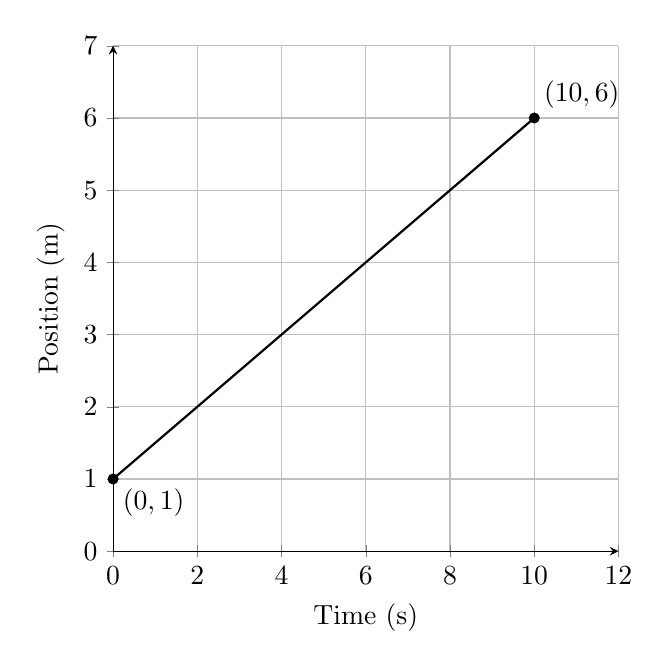
\begin{tikzpicture}
\begin{axis}[axis lines=left,
    width=8cm, height=8cm,
    ymin=0, ymax=7,
    xmin=0, xmax=12,
    ylabel = {Position (m)},
    xlabel = {Time (s)},
    grid=both,
    ytick={0,1,...,7},
    clip=false
]
\addplot[mark=none,thick,
    ]
    coordinates {
    (0,1)(10,6)
    };
    \fill (0,1) circle (2pt) node[below right] {$(0,1)$};
    \fill (10,6) circle (2pt) node[above right] {$(10,6)$};
\end{axis}
\end{tikzpicture}
\captionsetup{type=figure,margin=1in}
\captionof{figure}{A position vs.~time graph representing constant motion (that is, constant speed).}
\label{Ujz7ke}
\end{center}

 (a) The first given coordinate is $(0,1)$. Since time is on the $x$-axis and position is on the $y$-axis, the coordinate $(0,1)$ means that at a time of 0 seconds, Woody's (initial) position is at 1 meter. Therefore, his initial position is 

\begin{equation*}
    d_i = \SI{1}{m}
\end{equation*}

(b) Likewise, the second coordinate $(10,6)$ indicates that at a time of 10 seconds, his position changed to 6 meters, so his final position is

\begin{equation*}
    d_f = \SI{6}{m}
\end{equation*}

The straight line between these 2 coordinates on a position vs.~times graph  signify that Woody traveled with \textit{constant} motion---that is, with a constant speed or velocity.

\hrule

\begin{example} \label{KcfJbJ}
    Calculate the displacement of Woody, from Example \ref{jS4CBO}. 
\end{example}

 In Example \ref{jS4CBO}, we interpreted the position vs.~time graph (Figure \ref{Ujz7ke}) as indicating that Woody's initial and final positions are

\begin{equation*}
    d_i = \SI{1}{m} \quad \text{and} \quad d_f = \SI{6}{m}
\end{equation*}

By Equation \eqref{DV73y9}, therefore, his displacement is

\begin{equation*}
    \Delta d = d_f - d_i = 6 - 1 = 5
\end{equation*}

Therefore, Woody's displacement across the 10-second time interval, is 5 meters.

\hrule

\begin{example}
    Calculate the average velocity of Woody, from Example \ref{jS4CBO}. 
\end{example}

 As noted in Example \ref{jS4CBO}, the straight line between the end points indicates that Woody travels with constant motion, or constant velocity. Thus, even though the graph is labeled ``position vs.~time,'' it is nevertheless possible to calculate speed and velocity information. In Example \ref{KcfJbJ}, we calculated that Woody's displacement is 5 meters:

\begin{equation*}
    \Delta d = \SI{5}{m}
\end{equation*}

Furthermore, from Figure \ref{Ujz7ke}, the time interval during the displacement is 10 seconds:

\begin{equation*}
    \Delta t = \SI{10}{s}
\end{equation*}

Therefore, by Equation \eqref{Elg0tf}, the average velocity is displacement divided by elapsed time:

\begin{equation*}
    \bar{v} = \frac{\Delta d}{\Delta t} = \frac{5}{10} = 0.5
\end{equation*}

Woody's average velocity is 0.5 meters per second.

\hrule

\begin{example} \label{Xpi5rU}
Consider the position vs.~time graph below, which describes the motion of a pedestrian over time. What is the pedestrian's displacement across the entire time interval?
\end{example}

\begin{center}
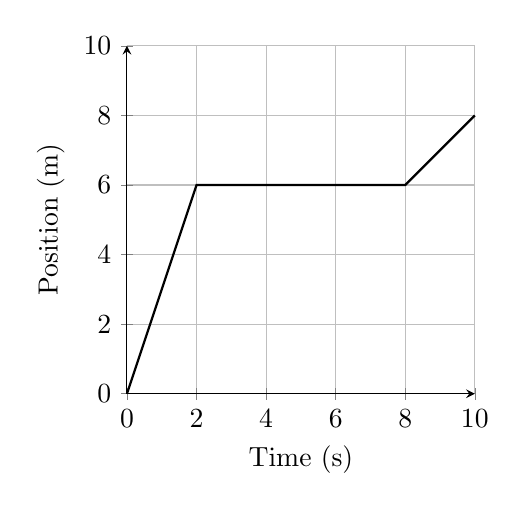
\begin{tikzpicture}
\begin{axis}[
    width=6cm,height=6cm,
    clip=false,
    axis lines=left,
    xlabel={Time (s)},
    ylabel={Position (m)},
    xmin=0,xmax=10,ymin=0,ymax=10,
    ymajorgrids=true,
    xmajorgrids=true,
]
\addplot[color=black,thick]
    coordinates{
        (0,0)(2,6)(8,6)(10,8)
    };
\end{axis}
\end{tikzpicture}
\end{center}

 We are given the pedestrian's initial position, final position, and elapsed time: $d_i = \SI{0}{m}$, $d_f = \SI{8}{m}$, and $\Delta{t} = \SI{10}{s}$. The unknown is displacement. By Eq.~(\ref{DV73y9}), displacement is

\begin{equation*}
    \Delta d = d_f - d_i = 8 - 0 = \SI{+8}{m}
\end{equation*}

The pedestrian's displacement is 8 meters from the origin.

\hrule

\begin{example}
    For the graph in Example \ref{Xpi5rU}, calculate the pedestrian's average velocity in the last 2 seconds of motion.
\end{example}

 We are given initial and final positions and initial and final times for the last 2 seconds of motion: $d_i = \SI{6}{m}$, $d_f = \SI{8}{m}$, $t_i = \SI{8}{s}$, and $t_f = \SI{10}{s}$. The unknown is average velocity during this time interval: $\bar{v} =\ ?$ By Eq.~(\ref{Elg0tf}), average velocity is

\begin{equation*}
    \bar{v} = \frac{d_f - d_i}{t_f - t_i} = \frac{8 - 6}{10 - 8} = \SI{1}{m/s}
\end{equation*}

The pedestrian's average velocity is 1 meter per second.

\hrule

\begin{example}
    Calculate average velocity in the graph below for time elapsed from 10 seconds to 40 seconds.
\end{example}

\begin{center}
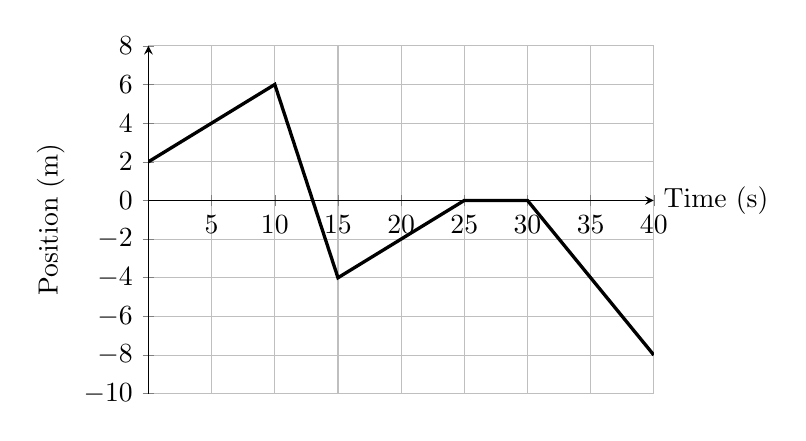
\begin{tikzpicture}
\begin{axis}[width=8cm,height=6cm,
    axis y line=left, 
    axis x line=center,
    every axis x label/.style={at={(current axis.right of origin)},anchor=west},
    xlabel = Time (s),
    ylabel = Position (m),
    ymin=-10, ymax=8,
    xmin=0, xmax=40,
    ytick={-10,-8,...,8},
    xtick={0,5,10,...,40},
    ymajorgrids=true,
    xmajorgrids=true,
]
    \addplot[color=black, very thick,
        ]
        coordinates {
        (0,2)(10,6)(15,-4)(20,-2)(25,0)(30,0)(40,-8)
        };
\end{axis}
\end{tikzpicture}
\end{center}

 From the graph, which seems complicated, we simply see that we are given initial and final positions and initial and final times from 10 to 40 seconds:

\begin{equation*}
    d_i = \SI{6}{m}\ , \quad
    d_f = \SI{-8}{m}\ , \quad
    t_i = \SI{10}{s}\ , \quad
    t_f = \SI{40}{s}
\end{equation*}

The unknown is average velocity across this time interval: $\bar{v} =\ ?$ The given and unknown quantities are related by Equation \eqref{Elg0tf},

\begin{equation*}
    \bar{v} = \frac{\Delta{d}}{\Delta{t}} = \frac{d_f - d_i}{t_f - t_i}
\end{equation*}

Substituting given values leads to

\begin{equation*}
    \bar{v} = \frac{-8-6}{40-10}
\end{equation*}

This simplifies to

\begin{equation*}
    \bar{v} = \frac{-14}{30} = -\SI{0.47}{m/s}
\end{equation*}

The average velocity is $-0.47$ meters per second, or 0.47 meters per second to the left.

% \begin{multicols}{2}

\vspace{1em}

\hrule




% \end{multicols}

\hrule

\section{Velocity vs.~Time Graphs} \label{EOqf0D}

A \relax{velocity vs. time graph} is like a position vs.~times graph but with velocity on the $y$-axis. These $v$ vs.~$t$ graphs show when objects speed up, slow down, or move at a constant speed. This entire unit has involved objects traveling at constant or zero velocity. In the next unit, we will explore objects that change velocity over time. But first, let's revisit the average velocity equation.

\begin{example}
    Solve the average velocity equation \eqref{Elg0tf} algebraically for displacement.
\end{example}

 Recall that, by Equation \eqref{Elg0tf}, average velocity is displacement over time:

\begin{equation*}
    \bar{v} = \frac{\Delta{d}}{\Delta{t}}
\end{equation*}

We solve for displacement $\Delta{d}$ as follows:

\begin{align*}
    \textbf{Write $\Delta{d}$ on left} \qquad & \frac{\Delta{d}}{\Delta{t}} = \bar{v}\\[1ex]
    \textbf{Multiply by time} \qquad & \frac{\Delta{d}}{\cancel{\Delta{t}}} \times \textcolor{red}{\cancel{\Delta{t}}} = \bar{v} \times \textcolor{red}{\Delta{t}}\\[1ex]
    \textbf{Simplify} \qquad & \Delta{d} = \bar{v}\,\Delta{t}
\end{align*}

Therefore, displacement is average velocity multiplied by time:

\begin{equation} \label{a71bdD}
    \Delta{d} = \bar{v}\,\Delta{t}
\end{equation}

That is, displacement is the product of average velocity and time. This idea plays an essential role in velocity vs.~times graphs and in the next example.

\begin{example} \label{uuZRlv}
The velocity vs.~time graph below represents the motion of a golf cart traveling at a constant 15 meters per second over a time interval of 6 seconds. What is the cart's displacement throughout the time interval?
\end{example}

\begin{center}
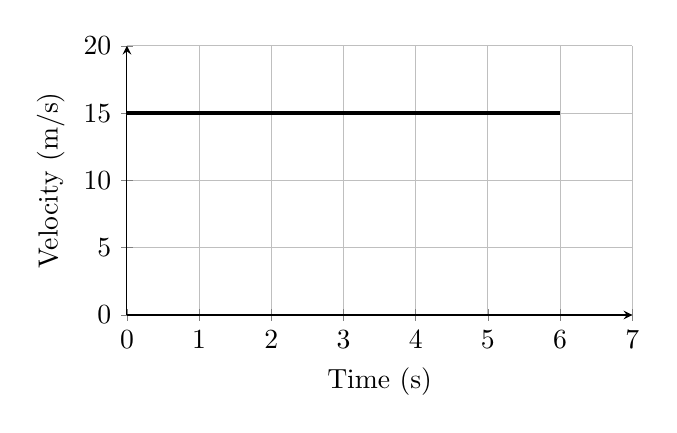
\begin{tikzpicture}
\begin{axis}[axis lines=left,
        width=8cm,height=5cm,
        ymin=0, ymax=20,
        xmin=0, xmax=7,
        ylabel = Velocity (m/s),
        xlabel = Time (s),
        grid=both,
        ytick={0,5,...,20},
    ]
    \addplot[black, very thick,
        ]
        coordinates {
        (0,15)(6,15)
        };
\end{axis}
\end{tikzpicture}
\captionsetup{type=figre,margin=1in,font=scriptsize}
\captionof{figure}{A graph showing constant velocity over time.}
\label{paOxO0}
\end{center}

 Do you see how the line graph bounds a rectangular area, as shown below?

% Displacement is the area under the curve. The area bounded by the curve is a rectangle. The area ($A$) of a rectangle is given by its length ($l$) multiplied by its width ($w$): 



% \begin{equation*} 
%     A = l w 
% \end{equation*}

\begin{center}
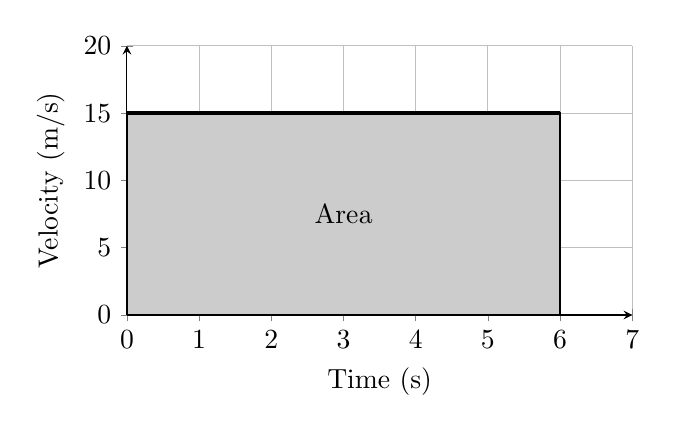
\begin{tikzpicture}
\begin{axis}[axis lines=left,
        width=8cm,height=5cm,
        ymin=0, ymax=20,
        xmin=0, xmax=7,
        ylabel = Velocity (m/s),
        xlabel = Time (s),
        grid=both,
        ytick={0,5,...,20},
    ]
    \fill[black!20] (axis cs: 0,0) rectangle (axis cs: 6,15) node[black,pos=0.5] {Area};
    \draw[black,thick] (axis cs: 0,0) rectangle (axis cs: 6,15);
    \addplot[color=black,
        very thick,
        ]
        coordinates {
        (0,15)(6,15)
        };
\end{axis}
\end{tikzpicture}
\captionsetup{type=figure,margin=1in,font=scriptsize}
\captionof{figure}{The area of a rectangle is bounded by a constant-velocity line graph.}
\label{5kJDXd}
\end{center}

The area of a rectangle is length multiplied by width:

\begin{equation} \label{ANqiK7}
    A = l w
\end{equation}

Because the ``width'' of the rectangle in Figure \ref{5kJDXd} is velocity and the ``length'' is time, the area must be velocity multiplied by time. But according to Equation \eqref{a71bdD}, the product of velocity and time is displacement. Therefore, by calculating the area of the rectangle, we are simultaneously calculating the gold cart's displacement. This becomes more apparent when you compare Equations \eqref{ANqiK7} and \eqref{a71bdD}.

\vspace{1em}

The width is a velocity of \SI{15}{m/s}, and the length is a time of \SI{6}{s}. So, the area of the rectangle is 

\begin{equation*}
    A = 6 \times 15 = 90
\end{equation*}

Therefore, the object's displacement is 90 meters to the right of the origin. Although ``displacement'' does not appear in the title of a ``velocity vs.~time'' graph, it is nevertheless possible to calculate displacement information from these graphs.

\hrule

The idea discovered in Example \ref{uuZRlv} that displacement is the area under a velocity vs.~times graph is not unique to rectangles: the area bounded by any shape under the graph is displacement.

\begin{mdframed}[backgroundcolor=black!10]
    \centering
    \textbf{The area bounded by a curve in a velocity vs.~time graph is displacement.}
\end{mdframed}

\begin{example} \label{HjmJqM}
    A golf ball rolls to the left at a constant speed, strikes a wall after 3 seconds, and rolls in the opposite direction at a constant but slower speed. It's motion is described in the graph below. What is the ball's displacement from it's original position across its 10 seconds of motion?
\end{example}

\begin{center}
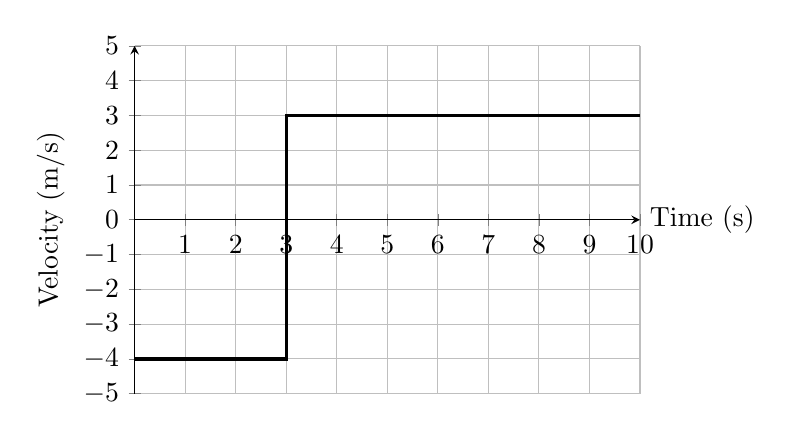
\begin{tikzpicture}
\begin{axis}[width=8cm,height=6cm,
    axis y line=left, 
    axis x line=center,
    every axis x label/.style={at={(current axis.right of origin)},anchor=west},
    xlabel = Time (s),
    ylabel = Velocity (m/s),
    ymin=-5, ymax=5,
    xmin=0, xmax=10,
    ytick={-5,-4,...,5},
    xtick={0,1,...,10},
    ymajorgrids=true,
    xmajorgrids=true,
]
    \addplot[color=black, very thick,
        ]
        coordinates {
        (0,-4)(3,-4)(3,3)(10,3)
        };
\end{axis}
\end{tikzpicture}
\end{center}

 Two rectangles of areas $A_1$ and $A_2$ are bounded by the curve:

\begin{center}
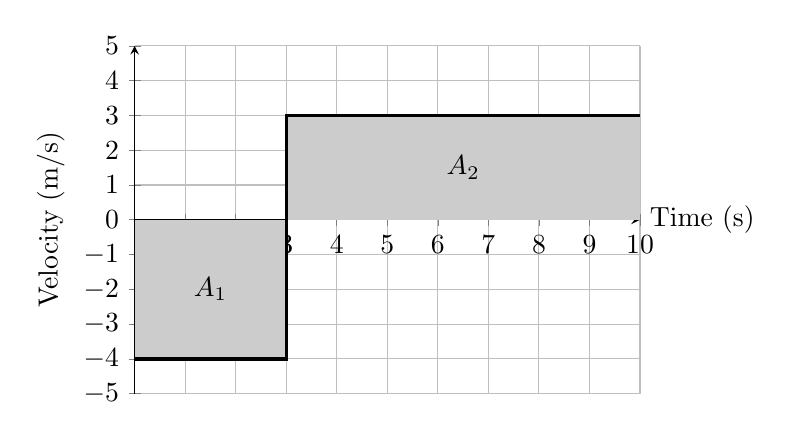
\begin{tikzpicture}
\begin{axis}[width=8cm,height=6cm,
    axis y line=left, 
    axis x line=center,
    every axis x label/.style={at={(current axis.right of origin)},anchor=west},
    xlabel = Time (s),
    ylabel = Velocity (m/s),
    ymin=-5, ymax=5,
    xmin=0, xmax=10,
    ytick={-5,-4,...,5},
    xtick={0,1,...,10},
    ymajorgrids=true,
    xmajorgrids=true,
]
    \fill[color=black!20] (0,-4) rectangle (3,0) node[black,pos=0.5] {$A_1$};
    \fill[color=black!20] (3,0) rectangle (10,3) node[black,pos=0.5] {$A_2$};
    \addplot[color=black, very thick,
        ]
        coordinates {
        (0,-4)(3,-4)(3,3)(10,3)
        };

\end{axis}
\end{tikzpicture}
\end{center}

Note that since the first rectangle is below the time axis ($x$-axis), in the negative velocity region, $A_1$ is a numerically negative area\footnote{Technically, in geometry areas cannot be negative, but we will ignore that fact for now.}. This solution develops like Example \ref{uuZRlv}. 

\vspace{1em}

The length and width of $A_1$ are 3 and $-4$, respectively, so by Equation \eqref{ANqiK7} the area is

\begin{equation*}
    A_1 = l w = 3\times (-4) = -12
\end{equation*}

Thus, area $A_1$ represents a displacement of $-12$ meters, which is consistent with the fact that the ball initially moves to the left. The second rectangle has a length of 7, since time elapsed from 3 to 10 seconds, and a width of 3, so the area is 

\begin{equation*}
    A_2 = 7 \times 3 = 21  
\end{equation*}

or a displacement of 21 meters to the right. The total displacement is found by summing the two areas as

\begin{equation*}
    A = A_1 + A_2 = -12 + 21 = 9
\end{equation*}

The golf ball traveled a total distance of 33 meters (12 + 21), but since it moved first to the left and then to the right, its overall displacement from the origin is 9 meters to the right.

\hrule

\section{Momentum and Kinetic Energy} \label{yUPGRH}

So far, we have defined the following physical quantities: position, distance, displacement, time, speed and velocity. Now we will define three more quantities---momentum and kinetic energy, both of which depend on a third quantity, mass. \relax{mass} is the quantity of matter in a substance and is measured in kilograms (kg). 

\vspace{1em}

\relax{momentum} ($p$) is the product of a system's mass and its velocity:

\begin{equation} \label{L05jSw}
    p = m v
\end{equation}

The SI units of momentum are the kilogram-meter per second (\SI{}{kg\,m/s}).

\begin{center}
    \begin{tabular}{cl|cl}
    \hline
    \textbf{Symbol} & \textbf{Quantity} & \textbf{SI Unit} & \textbf{Unit Symbol}  \\
    \hline\hline
    \rule{0pt}{2.5ex}
        $p$ & momentum & kilogram meter per second & \SI{}{kg\,m/s}\\
        $m$ & mass & kilogram & kg\\
        $v$ & velocity & meter per second & m/s\\
    \hline
    \end{tabular}
\end{center}

Equation \eqref{L05jSw} suggests that momentum is directly proportional to the object's mass ($m$) and velocity ($v$). Therefore, the greater an object's mass or the greater its velocity, the greater its momentum. A large, fast-moving object has greater momentum than a smaller, slower object. 

\begin{example} \label{lMBh9H}
    Calculate the momentum of a 110-kg \href{https://youtu.be/hxMaoFcYSrw}{football player} running at \SI{8}{m/s}.
\end{example}

 We are given mass and velocity: $m = \SI{110}{kg}$ and $v = \SI{8}{m/s}$. We want to find momentum: $p =\ ?$ By Eq.~(\ref{L05jSw}), momentum is mass times velocity:

\begin{equation*}
    p = m v = (110)(8) = \SI{880}{kg\,m/s} 
\end{equation*}

\hrule

\vspace{1em}

\relax{kinetic energy} is the energy of motion. Like momentum, it depends on an object's mass and velocity but is calculated using the following equation:

\begin{equation} \label{s57crz}
    \mathrm{KE} = \frac{1}{2} m v^2 
\end{equation}

The SI unit of kinetic energy is the joule (J).

\begin{center}
    \begin{tabular}{cl|cl}
    \hline
    \textbf{Symbol} & \textbf{Quantity} & \textbf{SI Base Unit} & \textbf{Unit Symbol}  \\
    \hline\hline
    \rule{0pt}{2.5ex}
        $\mathrm{KE}$ & kinetic energy & joule & J\\
        $m$ & mass & kilogram & kg\\
        $v$ & velocity & meter per second & m/s\\
    \hline
    \end{tabular}
\end{center}

\begin{example} \label{5qVtmV}
Chris Farley runs to the stage at \SI{4.0}{m/s}. If his mass is \SI{134}{kg}, what is his kinetic energy?
\end{example}

 We are given Farley's mass and velocity: $m = \SI{134}{kg}$ and $v =  \SI{4.0}{m/s}$. The unknown we are finding is kinetic energy: $\mathrm{KE} =\ ?$. By Eq.~(\ref{s57crz}),

\begin{equation*}
    \mathrm{KE} = \frac{1}{2} m v^2 = \frac{1}{2} \left(\SI{134}{kg}\right) \left(\SI{4.0}{m/s}\right)^2 = \SI{1072}{J}
\end{equation*}

\hrule

\begin{mdframed}[backgroundcolor=black!10]
\textbf{Calculator tip:} When using a calculator, don't use \texttt{1/2}. Instead, use \texttt{0.5}. 
\end{mdframed}

\begin{example} \label{PUlJG6}
The kinetic energy of a 60-kg skater is \SI{5880}{J}. What is her velocity?
\end{example}


 We are given the skater's kinetic energy and mass: $\mathrm{KE} = \SI{5880}{J}$ and $m = \SI{60}{kg}$. The unknown we are looking for is the skater's velocity: $v =\ ?$ These three quantities are related by Equation (\ref{s57crz}) as

\begin{equation*}
    \mathrm{KE} = \frac{1}{2} m v^2
\end{equation*}

We can solve this equation for velocity ($v$) via the following steps:

\begin{align*}
    \textbf{Write $v$ on left} \qquad & \frac{1}{2} m v^2 = \mathrm{KE}\\[0.5ex]
    \textbf{Substitute given quantities} \qquad & \frac{1}{2} \cdot 60 \cdot v^2 = 5880\\[0.5ex]
    \textbf{Multiply $\frac{1}{2}$ by 60} \qquad & 30\,v^2 = 5880\\[0.5ex]
    \textbf{Divide by 30} \qquad & \frac{\cancel{30}\,v^2}{\textcolor{red}{\cancel{30}}} = \frac{5880}{\textcolor{red}{30}}\\[0.5ex]
    \textbf{Simplify} \qquad & v^2 = 196\\[0.5ex]
    \textbf{Take square root} \qquad & \sqrt{v^2} = \sqrt{196}\\[0.5ex]
    \textbf{Simplify} \qquad & v = \SI{14}{m/s}\\
\end{align*}

Therefore, the skater's speed is 14 meters per second.

\hrule

\section{Exercises}

\begin{center}
    \begin{tikzpicture}
    \begin{axis}[width=15cm,
        axis lines = left,
        axis y line=none,
        xlabel = {Position (m)},
        ymin=0, ymax=12, 
        xmin=-10, xmax=10,
        xtick={-10,-8,...,12},
        clip=false,
        ]
        \node[above] at (-9,0) {\Springtree[3]};
        \node[above] at (7,0) {\huge \faHome};
        \node[above] at (4,0) {\Strichmaxerl[2.5]} ;
    \end{axis}
    \end{tikzpicture}
\end{center}

\begin{exercise} \label{kE0eEH}
    Find the position of (a) the person, (b) the tree, and (c) the house.
\end{exercise}

\begin{exercise} \label{dOncsX}
    The person walks to the house, then to the tree. What is their total distance traveled?
\end{exercise}

\begin{exercise} \label{Ka0olk}
    The person walks to the house, then to the tree. What is the person's displacement?
\end{exercise}

\begin{exercise}
    If the figure above shows the person's final position, and if they started at the house, what is their displacement?
\end{exercise}

\hrule

\vspace{1em}

\textbf{\ref{PTZXm9}--\ref{9nlNcq}} Emma Walker undergoes the three displacements shown below. Assume right is the positive direction.

\begin{center}
    \begin{tikzpicture}
    \begin{axis}[width=15cm,
        axis lines = left,
        axis y line=none,
        axis x line=none,
        xlabel = {Position (m)},
        ymin=0, ymax=12, 
        xmin=-15, xmax=75,
        xtick={-10,-8,...,12},
        clip=false,
        ]
        \node[above] at (0,0) {\Strichmaxerl[2.5]};
        \draw[->] (0,1) -- ++(axis direction cs: 48,0) node[above,pos=0.5] {\SI{48}{m}};
        \draw[->] (48,1.7) -- ++ (axis direction cs: -60,0) node[above,pos=0.5] {\SI{60}{m}};
        \draw[->] ({48-60},2.4) -- ++(axis direction cs: 85,0) node[above,pos=0.5] {\SI{85}{m}};
    \end{axis}
    \end{tikzpicture}
\end{center}

\begin{exercise} \label{PTZXm9}
    What is the total distance traveled by Emma?
\end{exercise}

\begin{exercise} \label{9nlNcq}
    What is Emma's total displacement?
\end{exercise}


\begin{exercise}
    Which of the following does your car's odometer record: distance or displacement?
\end{exercise}

\begin{exercise}
    Is distance a scalar or a vector?
\end{exercise}

\begin{exercise}
    Is displacement a scalar or a vector?
\end{exercise}

\begin{exercise}
    Provide at least 3 differences between distance and displacement.
\end{exercise}

\begin{exercise}
    Calculate Rodrigo's displacement, from Example~\ref{4Li1vK}, using the vector sum method that was modeled in Example~\ref{LBLwIS}.
\end{exercise}

\begin{exercise}
    Calculate Norma's displacement, from Example~\ref{mAnrq8}, using the vector sum method that was modeled in Example~\ref{LBLwIS}.
\end{exercise}

\begin{exercise} \label{xs4oMq}
A dog walks 14 meters to the east and then 20 meters back to the west.  (a) Draw a sketch of the dog's trip. (b) Calculate the distance traveled. (c) Calculate the dog's displacement. (\textit{Hint}: Let east be the positive direction.) (d) What is the magnitude of his displacement?
\end{exercise}


\hrule

\vspace{1em}

In a coordinate system in which the direction to the right is positive, Morgan walks 35 meters to the left, 18 meters to the right, and then 26 meters to the left.

\begin{exercise} \label{3rT1wE}
What distance does Morgan travel?
\end{exercise}

\begin{exercise} \label{0NkeX1}
What is Morgan's displacement?
\end{exercise}

\hrule

\vspace{1em}

Nimzy the cat moves 16 meters eastward, then 7 meters westward, and finally 3 meters eastward.

\begin{exercise} \label{umzXid}
    What total distance does Nimzy travel?
\end{exercise}

\begin{exercise} \label{CO3yuB}
    What is the magnitude of the Nimzy's displacement?
\end{exercise}

\begin{exercise} \label{2O3f3z}
    What is the direction of Nimzy's displacement?
\end{exercise}

\hrule

\vspace{1em}

\textbf{\ref{raIRVr}--\ref{Dxhphh}} Suppose you walk halfway around a circular track of radius \SI{63.67}{m}, as shown in the figure below.

\begin{center}
\begin{tikzpicture}
\begin{axis}[width=5cm,height=5cm,
    axis equal,
    ticks=none,
    clip=false,
    xmin=-1,xmax=1,ymin=-1,ymax=1,
    axis lines=center,
    axis line style={draw=none},
]
    \fill (-1,0) circle (2pt) node[left] {start};
    \fill (1,0) circle (2pt) node[right] {end};
    \draw[->,thick] (-1,0) arc (180:2:1);
    \draw[dashed] (1,0) arc (0:-180:1);
\end{axis}
\end{tikzpicture}
\end{center}

\begin{exercise} \label{raIRVr}
    What total distance do you travel?
\end{exercise}

\begin{exercise} \label{Dxhphh}
    Calculate your displacement.
\end{exercise}

%%%%%%%%

\textbf{\ref{qquil7}--\ref{cIfbMu}} Quinn jogs back and forth in one dimension, undergoing several displacements in the following sequence: 40 meters east, 24 meters west, \SI{36}{m} east, \SI{49}{m} west, \SI{14}{m} east, and finally \SI{45}{m} west. The total elapsed time of her trip is 33 seconds. Assume east is the positive direction.

\begin{exercise} \label{qquil7}
    Draw a diagram for Quinn's trip like Figure \ref{vds9fx}. Include labels and arrows showing the displacements.
\end{exercise}

\begin{exercise} \label{c7YaTG}
    What total distance does Quinn travel?
\end{exercise}

\begin{exercise} \label{ASXgWQ}
    What is Quinn's average speed?
\end{exercise}

\begin{exercise} \label{iG7rDo}
    Calculate Quinn's displacement.
\end{exercise}

\begin{exercise} \label{cIfbMu}
    Find Quinn's average velocity.
\end{exercise}

\hrule

\begin{exercise} \label{JYqHaE}
    Is it possible to determine a car's instantaneous velocity from just the speedometer reading? Explain.
\end{exercise}

\begin{exercise} \label{EeYgx7}
A pitcher throws a baseball from the pitcher's mound to home plate in \SI{0.46}{s}. The distance between the mound and home plate is \SI{18.4}{m}. What is the average speed of the baseball?
\end{exercise}

\begin{exercise} \label{Zj7dfC}
    A soccer ball travels with an average speed of \SI{16}{m/s} for \SI{3.0}{s}. How far did the ball travel?
\end{exercise}

\hrule

\vspace{1em}

\begin{exercise} \label{ix2lKL}
Eduardo jogs with an average velocity of 6.1 meters per second east. What is his displacement after 75 seconds?
\end{exercise}


\begin{exercise} \label{BI1eOB}
If displacement is \SI{428}{m} west and average velocity is \SI{1.70}{m/s} west, what is the elapsed time?
\end{exercise}

%%%%%%%%%%%%%%%%%%

\begin{center}
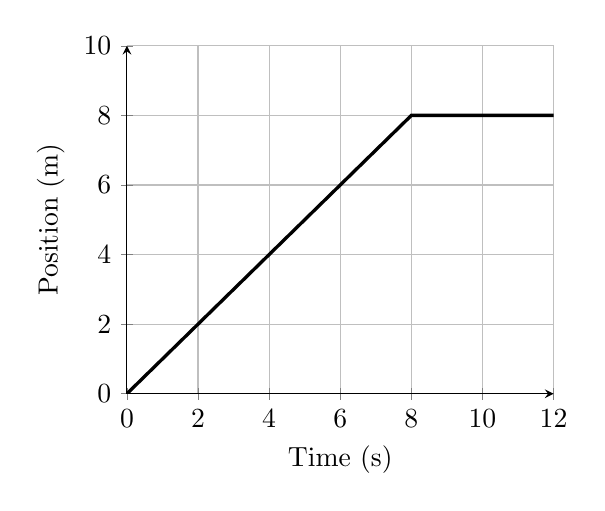
\begin{tikzpicture}
\begin{axis}[width=7cm, height=6cm,
        axis y line=left, 
        axis x line=left,
        ymin=0, ymax=10,
        xmin=0, xmax=12,
        ylabel = Position (m),
        xlabel = Time (s),
        grid=both,
        ytick={0,2,...,10}
    ]
    \addplot[color=black,very thick,
        ]
        coordinates {
        (0,0)(8,8)(10,8)(12,8)
        };
    \end{axis}
    \end{tikzpicture}
\end{center}

\begin{exercise} \label{WTBtZb}
    Find the initial position, final position, and displacement across the entire time interval.
\end{exercise}

\begin{exercise} \label{wqqrdf}
    Calculate displacement in the time interval from 4 to 12 seconds.
\end{exercise}

\begin{exercise} \label{HQaLcm}
    What is the average velocity in the last 6 seconds of motion?
\end{exercise}

\hrule

\vspace{1em}

Consider the graph below.

\begin{center}
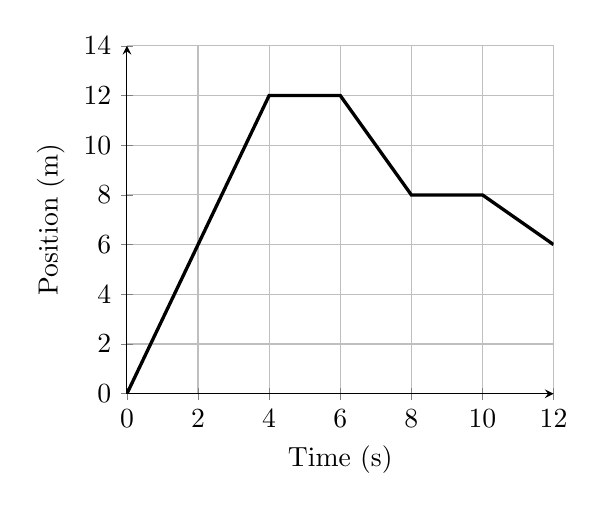
\begin{tikzpicture}
\begin{axis}[width=7cm,height=6cm,
    axis lines=left,
    ymin=0, ymax=14,
    xmin=0, xmax=12,
    ylabel = Position (m),
    xlabel = Time (s),
    grid=both,
    ytick={0,2,...,14}
]
\addplot[color=black,
    very thick,
    ]
    coordinates {
        (0,0)(2,6)(4,12)(6,12)(8,8)(10,8)(12,6)
    };
\end{axis}
\end{tikzpicture}
\end{center}

\begin{exercise} \label{hmsqqg}
    What is the runner's net displacement over the entire time interval?
\end{exercise}

\begin{exercise} \label{dixR7T}
    What is the runner’s average velocity over the entire time interval?
\end{exercise}

\begin{exercise} \label{YYxvX1}
   What is the average velocity in the first 4 seconds? 
\end{exercise}


\hrule

\vspace{1em}

Consider the graph below.

\begin{center}
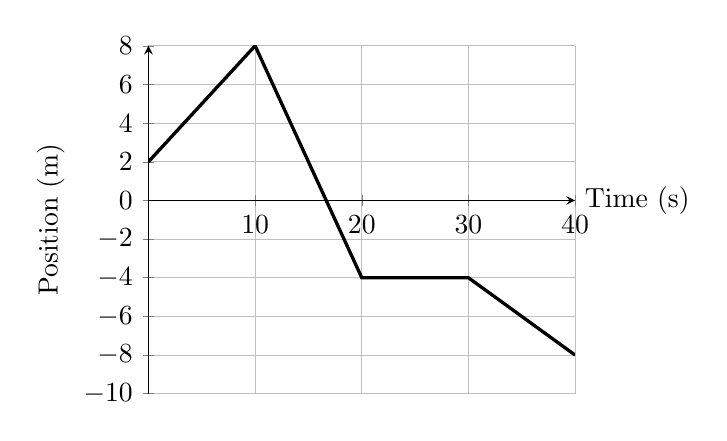
\begin{tikzpicture}
\begin{axis}[width=7cm,height=6cm,
    axis y line=left, 
    axis x line=center,
    every axis x label/.style={at={(current axis.right of origin)},anchor=west},
    xlabel = Time (s),
    ylabel = Position (m),
    ymin=-10, ymax=8,
    xmin=0, xmax=40,
    ytick={-10,-8,...,8},
    xtick={0,10,...,40},
    ymajorgrids=true,
    xmajorgrids=true,
]
    \addplot[color=black, very thick,
        ]
        coordinates {
        (0,2)(10,8)(20,-4)(30,-4)(40,-8)
        };
\end{axis}
\end{tikzpicture}
\end{center}

\begin{exercise} \label{5Wd4QG}
    What is the displacement over the entire time interval?
\end{exercise}


\begin{exercise} \label{OselF0}
   What is the displacement over the first 10 seconds? 
\end{exercise}


\begin{exercise} \label{ZRQnM6}
    What is the average velocity for the whole time period shown in the graph?
\end{exercise}

\begin{exercise} \label{fZtSlq}
    What is the velocity between 10 and 20 seconds?
\end{exercise}

%%%%%%%%%%%%%%%

\begin{exercise} \label{E3dHaa}
    Calculate the displacement of the object whose motion is represented by the graph.
\end{exercise}

\begin{center}
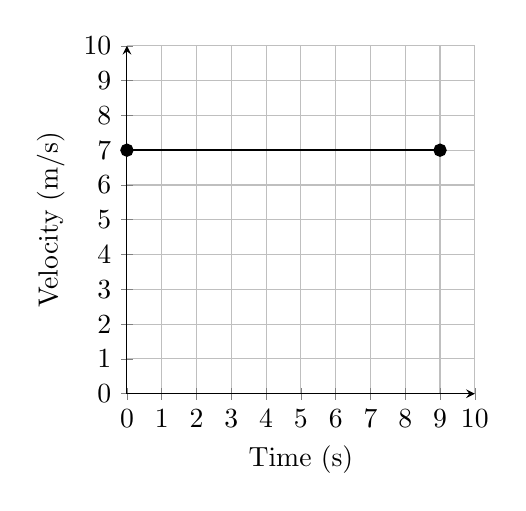
\begin{tikzpicture}
\begin{axis}[axis lines=left,
        width=6cm,height=6cm,
        ymin=0, ymax=10,
        xmin=0, xmax=10,
        ylabel = Velocity (m/s),
        xlabel = Time (s),
        grid=both,
        ytick={0,1,...,10},
        xtick={0,1,...,10}
    ]
    \addplot[thick,mark=*,
        ]
        coordinates {
        (0,7)(9,7)
        };
\end{axis}
\end{tikzpicture}
\end{center}

\begin{exercise} \label{1xi7hi}
    Calculate the total displacement of the object who's motion is represented by the graph below.
\end{exercise}

\begin{center}
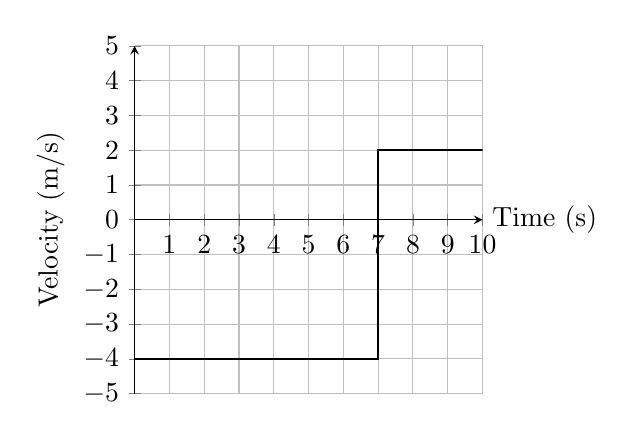
\begin{tikzpicture}
\begin{axis}[axis y line=left, 
        axis x line=center,
        width=6cm,height=6cm,
        ymin=-5, ymax=5,
        xmin=0, xmax=10,
        ylabel = Velocity (m/s),
        xlabel = Time (s),
        grid=both,
        ytick={-5,-4,...,5},
        xtick={0,1,...,10},
        every axis x label/.style={at={(current axis.right of origin)},anchor=west},
    ]
\addplot[mark=none,thick,
    ]
    coordinates {
    (0,-4)(7,-4)(7,2)(10,2)
    };
\end{axis}
\end{tikzpicture}
\end{center}

\begin{exercise}
    Calculate the average velocity of object whose motion is represented by the position vs.~time graph below. Then create a velocity vs.~time graph similar to the one in Figure \ref{paOxO0}.
\end{exercise}

\begin{center}
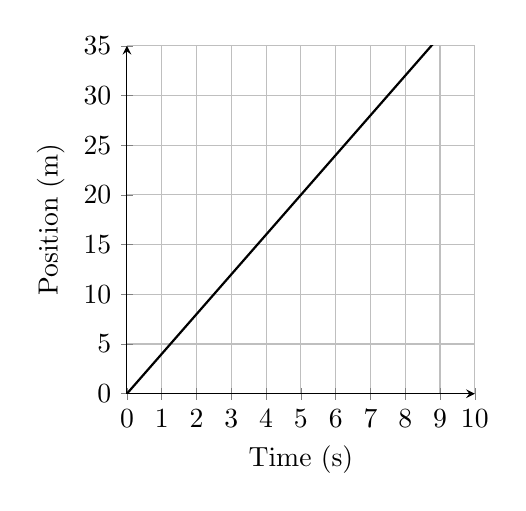
\begin{tikzpicture}
\begin{axis}[axis lines=left,
    width=6cm, height=6cm,
    ymin=0, ymax=35,
    xmin=0, xmax=10,
    ylabel = {Position (m)},
    xlabel = {Time (s)},
    grid=both,
    ytick={0,5,...,35},
    xtick={0,1,...,10},
    clip=true
]
\addplot[mark=none,thick,
    ]
    coordinates {
    (0,0)(10,40)
    };
\end{axis}
\end{tikzpicture}%
\hspace{1em}
\begin{tikzpicture}
\begin{axis}[axis lines=left,
    width=6cm, height=6cm,
    ymin=0, ymax=35,
    xmin=0, xmax=10,
    ylabel = {Velocity (m/s)},
    xlabel = {Time (s)},
    xtick={0,1,...,10},
    clip=true,
    every y tick label/.append style={white},  
    every y tick/.append style={white}]
]
\end{axis}
\end{tikzpicture}
\end{center}



%%%%%%%
% Momentum and Kinetic Energy:

\begin{exercise}
    Can a lighter object have more momentum than a heavier one? How?
\end{exercise}


\begin{exercise} \label{QDJrfn}
    Calculate the momentum of a 0.410-kg football thrown hard at a speed of \SI{25}{m/s}. Compare this momentum to the football player's momentum from Example \ref{lMBh9H} by calculating the ratio of the player's momentum to the ball's momentum, $p_{\text{player}}/p_{\text{ball}}$.
\end{exercise}

\begin{exercise} \label{9FyFRV}
    A \SI{5}{kg} bowling ball is rolled with a velocity of \SI{10}{m/s}. What is its momentum?
\end{exercise}


\begin{exercise} \label{5CHfrd}
    If an asteroid's mass and velocity are \SI{10}{kg} and \SI{11}{m/s}, kinetic energy?
\end{exercise}

\begin{exercise} \label{s9xduj}
    Calculate the kinetic energy of the bowling ball from Exercise \ref{9FyFRV}.
\end{exercise}

\begin{exercise} \label{pVdq3i}
    The kinetic energy of a a 5-kilogram object is 1200 joules. What is its speed?
\end{exercise}


\clearpage

\section{References \& Additional Resources}

Videos from the \textit{YouTube} channel \texttt{Khan Academy}:
\vspace{-1ex}

\begin{enumerate}
\setlength\itemsep{0.1ex}
    \item ``Distance and displacement introduction'' (\href{https://youtu.be/vQCkYm3v3aA}{https://youtu.be/vQCkYm3v3aA})
    \item ``Distance and displacement in one dimension'' (\href{https://youtu.be/w2mbvtpQKrM}{https://youtu.be/w2mbvtpQKrM})
    \item ``Intro to vectors \& scalars'' (\href{https://youtu.be/ihNZlp7iUHE}{https://youtu.be/ihNZlp7iUHE})
    \item ``Position-time graphs'' (\href{https://youtu.be/9XxzIoUQd78}{https://youtu.be/9XxzIoUQd78})
    \item ``Worked example: distance and displacement from position-time graphs'' (\href{https://youtu.be/az6i2qvI1E0}{https://youtu.be/az6i2qvI1E0})
    \item ``Average velocity and speed worked example'' (\href{https://youtu.be/Dzw2nLd7DFw}{https://youtu.be/Dzw2nLd7DFw})
    \item ``Instantaneous speed and velocity'' (\href{https://youtu.be/pfTTHx9kCHk}{https://youtu.be/pfTTHx9kCHk})
    \item ``Why distance is area under velocity-time line'' (\href{https://youtu.be/d-_eqgj5-K8}{click here})
    \item Practice: Slope from graph (\href{https://www.khanacademy.org/math/algebra/x2f8bb11595b61c86:linear-equations-graphs/x2f8bb11595b61c86:slope/e/slope-from-a-graph?modal=1}{click here})
    \item Practice: Slope from two points (\href{https://www.khanacademy.org/math/algebra/x2f8bb11595b61c86:linear-equations-graphs/x2f8bb11595b61c86:slope/e/slope-from-two-points?modal=1}{click here})
\end{enumerate}

Other resources:
\vspace{-1ex}
\begin{enumerate}
\setlength\itemsep{0.1ex}
    \item \textit{OpenStax Simulations}: ``Moving Man'' (\href{https://archive.cnx.org/specials/e2ca52af-8c6b-450e-ac2f-9300b38e8739/moving-man/}{click here})
    \item \textit{YouTube}: ``Introduction to Displacement and the Difference between Displacement and Distance'' by \texttt{Flipping Physics} (\href{https://youtu.be/uTQ4_AOae1g}{click here})
    \item \textit{YouTube}: ``Maths Bitesize -- The DST Triangle'' (\href{https://youtu.be/8glfUANjBbY}{https://youtu.be/8glfUANjBbY})
    \item \textit{PhET Simulation}: ``Graphing Lines'' (\href{https://phet.colorado.edu/sims/html/graphing-lines/latest/graphing-lines_en.html}{click here})
    \item \textit{Math Whiteboard} (\href{https://www.mathwhiteboard.com/whiteboard/}{https://www.mathwhiteboard.com/whiteboard/})
\end{enumerate}

\clearpage
\section{Answers to Select Exercises}

\ref{kE0eEH}. (a) 4 meters \hspace{1em} (b) \SI{+7}{m} \hspace{1em} (c) \SI{-9}{m}\\
\ref{dOncsX}. \SI{19}{m}\\
\ref{Ka0olk}. \SI{-13}{m}\\
\ref{xs4oMq}. (b) \SI{34}{m} \hspace{2em} (c) $-\SI{6}{m}$ or \SI{6}{m} west \hspace{2em} (d) \SI{6}{m}\\ 
\ref{3rT1wE}. 79 meters\\
\ref{0NkeX1}. \SI{-43}{m}\\
\ref{umzXid}. 26 meters\\
\ref{CO3yuB}. \SI{12}{m}\\
\ref{2O3f3z}. East\\
\ref{c7YaTG}. 208 meters\\
\ref{ASXgWQ}. \SI{6.3}{m/s}\\
\ref{iG7rDo}. $-\SI{28}{m}$\\
\ref{cIfbMu}. $-\SI{0.85}{m/s}$\\
\ref{JYqHaE}. No, since a speedometer doesn't specify direction.\\
\ref{EeYgx7}. \SI{40.0}{m/s}\\
\ref{Zj7dfC}. \SI{48}{m}\\
\ref{ix2lKL}. \SI{458}{m} east\\
\ref{BI1eOB}. \SI{252}{m}\\
\ref{WTBtZb}. $d_i=\SI{0}{m/s}$, $d_f=\SI{8}{m}$, $\Delta{d} = +\SI{8}{m}$\\
\ref{wqqrdf}. \SI{4}{m}\\
\ref{HQaLcm}. $\SI[parse-numbers = false]{\frac{1}{3}}{m/s}$\\
\ref{hmsqqg}. \SI{6}{m}\\
\ref{dixR7T}. \SI{0.5}{m/s}\\
\ref{YYxvX1}. \SI{3}{m/s}\\
\ref{5Wd4QG}. $-\SI{10}{m}$\\
\ref{OselF0}. $+\SI{6}{m}$\\
\ref{ZRQnM6}. $-\SI{0.25}{m/s}$\\
\ref{fZtSlq}. $-\SI{1.2}{m/s}$\\
\ref{E3dHaa}. \SI{63}{m/s}\\
\ref{1xi7hi}. $-\SI{22}{m}$\\
\ref{QDJrfn}. (a) \SI{10.25}{kg\,m/s} \hspace{1em} (b) 85.9\\
\ref{9FyFRV}. \SI{50}{kg\,m/s}\\
\ref{5CHfrd}. \SI{605}{J}\\
\ref{s9xduj}. \SI{250}{J}\\
\ref{pVdq3i}. \SI{21.9}{m/s}


\end{document}



